\documentclass[a4paper]{article}
\usepackage{multicol}
\usepackage{pgfplots}
\usepackage{amsmath}
\usetikzlibrary{positioning}
\pgfplotsset{every axis legend/.append style={fill=none, draw=none}}
\pgfplotsset{compat=1.3}

\begin{document}
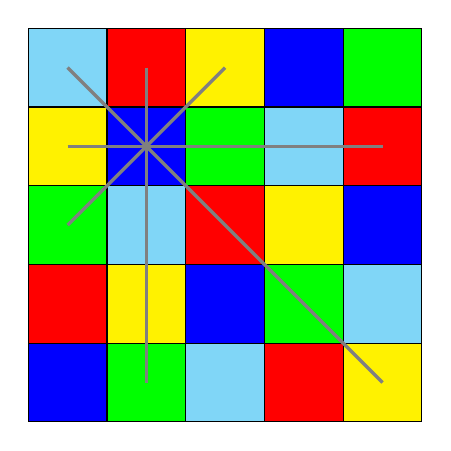
\begin{tikzpicture}
  [ sq1/.style={rectangle, draw=black, minimum size=10mm, fill=blue},
    sq2/.style={rectangle, draw=black, minimum size=10mm, fill=red},
    sq3/.style={rectangle, draw=black, minimum size=10mm, fill=green},
    sq4/.style={rectangle, draw=black, minimum size=10mm, fill=yellow},
    sq5/.style={rectangle, draw=black, minimum size=10mm, fill=cyan!50!white},
    line/.style={-, very thick, black!50}
  ]
  
  \node[sq1] at (0,0) {};
  \node[sq2] at (0,1) {};
  \node[sq3] (zerotwo) at (0,2) {};
  \node[sq4] (zerothree) at (0,3) {};
  \node[sq5] (zerofour) at (0,4) {};
  \node[sq3] (onezero) at (1,0) {};
  \node[sq4] at (1,1) {};
  \node[sq5] at (1,2) {};
  \node[sq1] at (1,3) {};
  \node[sq2] (onefour) at (1,4) {};
  \node[sq5] (twozero) at (2,0) {};
  \node[sq1] at (2,1) {};
  \node[sq2] at (2,2) {};
  \node[sq3] at (2,3) {};
  \node[sq4] (twofour) at (2,4) {};
  \node[sq2] at (3,0) {};
  \node[sq3] at (3,1) {};
  \node[sq4] (node2) at (3,2) {};
  \node[sq5] at (3,3) {};
  \node[sq1] at (3,4) {};
  \node[sq4] (fourzero) at (4,0) {};
  \node[sq5] at (4,1) {};
  \node[sq1] at (4,2) {};
  \node[sq2] (fourthree) at (4,3) {};
  \node[sq3] at (4,4) {};
  
  \draw [line] (zerofour.center) -- (fourzero.center);
  \draw [line] (zerotwo.center) -- (twofour.center);
  \draw [line] (onefour.center) -- (onezero.center);
  \draw [line] (zerothree.center) -- (fourthree.center);
\end{tikzpicture}

\vspace{40pt}

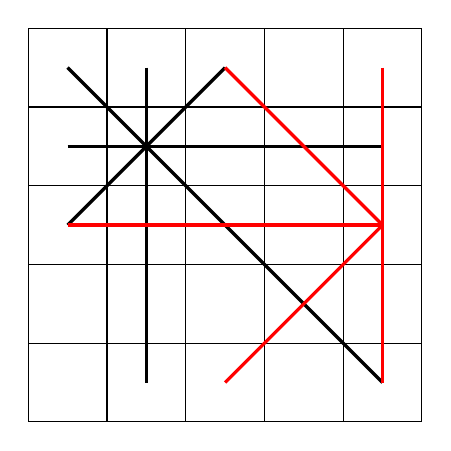
\begin{tikzpicture}
  [ sq1/.style={rectangle, draw=black, minimum size=10mm, fill=white},
    sq2/.style={rectangle, draw=black, minimum size=10mm, fill=white},
    sq3/.style={rectangle, draw=black, minimum size=10mm, fill=white},
    sq4/.style={rectangle, draw=black, minimum size=10mm, fill=white},
    sq5/.style={rectangle, draw=black, minimum size=10mm, fill=white},
    line1/.style={-, very thick, black},
    line2/.style={-, very thick, red}
  ]
  
  \node[sq1] at (0,0) {};
  \node[sq2] at (0,1) {};
  \node[sq3] (zerotwo) at (0,2) {};
  \node[sq4] (zerothree) at (0,3) {};
  \node[sq5] (zerofour) at (0,4) {};
  \node[sq3] (onezero) at (1,0) {};
  \node[sq4] at (1,1) {};
  \node[sq5] at (1,2) {};
  \node[sq1] at (1,3) {};
  \node[sq2] (onefour) at (1,4) {};
  \node[sq5] (twozero) at (2,0) {};
  \node[sq1] at (2,1) {};
  \node[sq2] at (2,2) {};
  \node[sq3] at (2,3) {};
  \node[sq4] (twofour) at (2,4) {};
  \node[sq2] at (3,0) {};
  \node[sq3] at (3,1) {};
  \node[sq4] (node2) at (3,2) {};
  \node[sq5] at (3,3) {};
  \node[sq1] at (3,4) {};
  \node[sq4] (fourzero) at (4,0) {};
  \node[sq5] at (4,1) {};
  \node[sq1] (fourtwo) at (4,2) {};
  \node[sq2] (fourthree) at (4,3) {};
  \node[sq3] (fourfour) at (4,4) {};
  
  \draw [line1] (zerofour.center) -- (fourzero.center);
  \draw [line1] (zerotwo.center) -- (twofour.center);
  \draw [line1] (onefour.center) -- (onezero.center);
  \draw [line1] (zerothree.center) -- (fourthree.center);
  
  \draw [line2] (fourfour.center) -- (fourzero.center);
  \draw [line2] (zerotwo.center) -- (fourtwo.center);
  \draw [line2] (twozero.center) -- (fourtwo.center);
  \draw [line2] (twofour.center) -- (fourtwo.center);
\end{tikzpicture}


\vspace{40pt}


\begin{equation*}
\begin{split}
\chi_{Q_5}(t) & = t^{25} -160t^{24} + 12400t^{23} -619000t^{22} + 22326412t^{21} -618664244t^{20} \\ & \quad 
+ 13671395276t^{19} -246865059671t^{18} + 3702615662191t^{17} \\ & \quad
-46639724773840t^{16} + 496954920474842t^{15}  -4497756322484864t^{14} \\ & \quad 
+ 34633593670260330t^{13} -226742890673713726t^{12} \\ & \quad 
+ 1258486280066672806t^{11} -5890734492089539317t^{10} \\ & \quad 
+ 23071456910844580538t^9 -74774310771536397886t^8 \\ & \quad  
+ 197510077615138465516t^7 -416375608854898733286t^6  \\ & \quad 
+ 680208675481930270860t^5 -824635131668099993614t^4 \\ & \quad 
+ 692768396747228503860t^3 -356298290543726707632t^2  \\ & \quad 
+ 83353136564448062208t
\end{split}
\end{equation*}
\end{document}
